\section{BPMN subset and execution semantics}
%\todo{Intro, subset, extensions}
In this paper, our main focus is on BPMN \textit{collaboration} models. According to the specification, they can contain \textit{processes} or \textit{choreographies}; we work with \textit{collaborative processes}.

Currently, we support a limited but representative set of elements from the BPMN specification, as summarized by table \ref{tab:sup_elem}. Notably, in addition to the Basic Modeling Elements of BPMN 2.0 (see \cite{bpmn}, p28), we also support message throw and catch events, which are of particular importance in collaborative settings. The table denotes those elements as ''stateful'' which have non-instantaneous execution semantics (as declared by the BPMN specification), and these will determine the structure of our execution state vector. In the context of this paper, we will refer to these elements as the ''executable'' ones in the BPMN subset we address.

%Some of the element types are considered executable. Others are there to control the execution flow. Executable elements' (like that of activities) state is tracked by this tool. The currently supported elements can be seen in table \ref{tab:sup_elem}.
\begin{table}
    \centering
    \caption{Supported BPMN modelling elements}
    \begin{tabular}{|c|c|c|}
        \hline
        \textbf{Element name} & \textbf{Notation} & \textbf{Stateful?}\\
        \hline
        \centerTable{Start event}
        &  \begin{tikzpicture} \node[event] (start) {}; \node[above=0.001 cm of start]{};\node[below=0.001 cm of start]{}; \end{tikzpicture} & \centerTable{no} \\
        \hline
        \centerTable{End Event}  &  \begin{tikzpicture} \node[end event] (end) {}; \node[above=0.01 cm of end]{};\node[below=0.01 cm of end]{};\end{tikzpicture} & \centerTable{no}\\
        \hline
        \centerTable{Activity} & \begin{tikzpicture} \node[task] (task) { Task }; \node[above=0.01 cm of task]{};\node[below=0.01 cm of task]{}; \end{tikzpicture} & \centerTable{yes} \\
        
        \hline
        Sequence flow & \begin{tikzpicture} \draw[-{Stealth[inset=0pt]}] (0,0) -- (1,0);\end{tikzpicture} & no \\
        \hline
        Message flow & \begin{tikzpicture} \draw[-{Stealth[open,inset=0pt]},dashed] (0.05,0) -- (1,0); \node[draw,circle,minimum size=0.1cm,inner sep=0pt, outer sep=0pt] at (0,0) {};\end{tikzpicture} & no \\
        \hline
        \centerTable{Parallel gateway} & \begin{tikzpicture} \node[gateway,node distance=6emg] (pg) {+}; \node[above=0.01 cm of pg]{};\node[below=0.01 cm of pg]{};\end{tikzpicture} & \centerTable{no} \\
        
        \hline
        \centerTable{Exclusive gateway} & \begin{tikzpicture}
            \node[gateway,node distance=4em,below=of start] (eg) {$\times$};
            \node[above=0.01 cm of eg]{};
            \node[below=0.01 cm of eg]{};
        \end{tikzpicture} & \centerTable{no} \\
        \hline
        Message & \begin{tikzpicture}
            \node[] at (0,0) {\faEnvelope[regular]} ; 
        \end{tikzpicture}& no \\
        \hline
        \centerTable{\makecell{Message Intermediate \\ Catch event  (executable)}} & 
        \begin{tikzpicture}
            \node[intermediate event,below=of eg,xshift=5em] (imc) {\faEnvelope[regular]};
             %\node[above=0.01 cm of imc]{};
             \node[below=0.1 cm of imc]{};
        \end{tikzpicture} & \begin{tikzpicture}
	        \node[](y){yes};
         \node[below=0.2 cm of y]{};
	    \end{tikzpicture}\\
        \hline
	    \centerTable{\makecell{Message Intermediate \\ Throw event  (executable)}} & 
	    \begin{tikzpicture}
		        \node[intermediate event,node distance=2em,below=of imc] (imt) {\faEnvelope};
		        %\node[above=0.01 cm of imt]{};
		        \node[below=0.1 cm of imt]{};
	    \end{tikzpicture} & \begin{tikzpicture}
	        \node[](y){yes};
         \node[below=0.2 cm of y]{};
	    \end{tikzpicture} \\
	    \hline
	    \begin{tikzpicture}
	        \node[](y){Pool};
         \node[below=0.15 cm of y]{};
	    \end{tikzpicture} & \begin{tikzpicture}[]
	        \node[minimum width=3cm,minimum height=1cm,draw,rectangle](b){};
	        \node[above=0.01 cm of b]{};
	        \node[rotate=90,draw,rectangle,left=0.2cm of b,xshift=0.5cm+\pgflinewidth,yshift=\pgflinewidth,minimum width=1cm] {\tiny Party1};
	    \end{tikzpicture} & \begin{tikzpicture}
	        \node[](y){no};
         \node[below=0.2 cm of y]{};
	    \end{tikzpicture} \\
	    \hline
	    \begin{tikzpicture}
	        \node[](y){Lane};
         \node[below=0.175 cm of y]{};
	    \end{tikzpicture} & \begin{tikzpicture}[]
	        \node[minimum width=2.5cm,minimum height=1cm,draw,rectangle](b){};
	        \node[above=0.01 cm of b]{};
	        
	        \node[rotate=90,draw,rectangle,left=0.2cm of b,xshift=0.5cm,yshift=-\pgflinewidth,minimum width=0.5cm] (a){\tiny A};
	        \node[rotate=90,draw,rectangle,left=0.2cm of b,xshift=0,yshift=-\pgflinewidth,minimum width=0.5cm] {\tiny B};
	        \node[rotate=90,draw,rectangle,left=0.4cm of a,xshift=0.5cm+\pgflinewidth,yshift=-\pgflinewidth,minimum width=1cm] (p){\tiny Party1};
	        
	        \draw[-] (p.south) --(b.east) ;
	    \end{tikzpicture} & \begin{tikzpicture}
	        \node[](y){no};
         \node[below=0.2 cm of y]{};
	    \end{tikzpicture} \\
	    \hline
    \end{tabular}
    \label{tab:sup_elem}
\end{table}


%We wanted to support at least the Basic Modeling Elements of BPMN 2.0\footnote{See Business Process Model and Notation, v2.0 \cite{bpmn}, page 28.}  to prioritize common components. We have also taken into account making modeling collaborations more executable. This is why We also included Message flows and Intermediate Message events. We chose these elements because these are the ones that are necessary and sufficient to model most of the relevant use cases.

\subsection{BPMN extensions and structural constraints}
%\label{bpmn_attr}
In order to capture properties that are necessary for our zero-knowledge approach, we added two types of extended attributes on top of the existing BPMN specification. On the one hand, a \texttt{zkp:publicKey} attribute is used to separate the tasks of different participants by attaching an EdDSA public key to a pool, a lane, or an executable element. Applying this attribute to an element directly or indirectly (e.g. through inclusion in a pool) is mandatory; however, there are no facilities for key overriding in the model hierarchy yet. The intended usage is to equip either pools or lanes with public keys.

\texttt{zkp:variables} extended attributes can be applied to \textit{activities}. These declare process instance global variables and that the variable may be written by that activity (reads are allowed for all activities). These variables can be used in expressions for exclusive gateways. The gateways support boolean expressions over these global variables.

Some constraints apply to the structure of the BPMN models currently admissible in our scheme.

\begin{itemize}
    \item We support binary gateways (at most two incoming/outgoing edges).
    \item Activities are \textit{atomic}; i.e., subprocesses are not supported.
    \item The model cannot contain loops; sequence and message flows must form a directed acyclic graph.
\end{itemize}

We plan to eliminate these constraints in the future; the required modifications of the state representation and the zkWF program construction are largely incremental.

\subsection{State representation}
Our notion of process instance execution state encompasses the following aspects (for the specific encoding in zkWF programs, please refer to the implementation).

\begin{itemize}
\item A vector $v$ of the current state of executable elements
\item The current values of \textit{global variables}
\item Hashes of the messages already sent in the process
\end{itemize}

Let us represent a business process $M$ as a tuple $(\vertices,\edges,\executables)$, where $\vertices$ is the set of non-flow model elements, $\edges$ is the set of model edges (flows), and $\executables\subset\vertices$ is the set of all executable elements in the business process. Then, $v$ is a vector of $|T|$ size and $\forall v_i \in v$ can have one of the following three values:

\begin{itemize}
    \item 0 (Inactive) -- The element has not been reached yet
    \item 1 (Active) -- The element is ready to be executed or is being executed by a party
    \item 2 (Completed) -- The execution of the element has been completed
\end{itemize}

Note that this state space model is a simplification, especially in terms of the full BPMN activity lifecycle; however, it is a reasonable simplification in the sense that it is of sufficient expressive power for important applications in our context (as we show later). Further research will investigate incorporating the full lifecycle model.

\subsection{Capturing token passing semantics}
As described by the standard, BPMN 2.0 models have token flow-based execution semantics. For the purposes of supporting a different ZKP use case, Aivo et al. \cite{toots_msc} introduce a technique for representing valid BPMN execution state changes through enumerating the possible composite token marking deltas of the elements upon stepping the process. 

Specifically, \cite{toots_msc} introduces an array $P$, where each element of $P$ is a list of token change and element identifier pairs -- essentially, $P$ enumerates the token changes for each allowed stepping of the BPMN model (not unlike Petri net incidence matrices do). 

We construct a very similar $P$ array and embed it into the zkWF program to enable checking whether a proposed state update is valid from the BPMN execution logic point of view.

Our token passing-based operational semantics is the following. Initially, we create a token for every start event and pass it to the first executable element connected to it. Each executable element has one incoming and one outgoing edge. When an executable event has a token, it is marked as ''active''. After completing the execution of the element, the element is marked as ''completed'', and we pass its token to the next executable element -- based on the token holder element's outgoing edge. This approach can be modelled as adding a token ($+1$) when we mark an executable event as ''active'', and we subtract this token ($-1$) when we mark the event as ''done''.

Gateways change the token flow differently. Parallel gateways can split a token on one end and merge them back together on the other end. Exclusive gateways can have many outgoing edges, but only one can be taken based on its assigned expression. A default outgoing edge can also be set, as described in the BPMN specification. End events can have multiple incoming edges but no outgoing edges. They mark the end of a token flow.

To limit the size of our version of array $P$ (necessary to ensure reasonable proof computation times), in our approach, a single step of a model can induce only three token changes at most. (Hence the structural restriction on parallel gateways.) Thus, the array $P$ describing one-step token marking changes for a model $M$ consists of 3-tuples with elements from the set $\mathcal{N}$: 

\begin{align}
    \mathcal{N}&=(+1, -1\}\times T)\cup \{(0,-1)\}
\end{align}

For $T$, we apply a simple integer encoding; the $-1$ in the ''no-token-change'' pair is a don't care placeholder.

%In general, $n\in\mathcal{N}$ is a pair of numbers describing a possible token change. The first component of the pair shows if the token is increased or decreased ($+1$ or $-1$). The second component $i$ marks the token change for the executable event $T[i]$.

%Since not every step consists of three token changes, $n$ can also be an "empty" token change. This is used as a placeholder and is marked as $(0,-1)$.

%Then, $P[i]$ shows how the process state can change in step $i$.

%\subsection{Limitations of BPMN models}
%\label{bpmn_limit}
%As We described in the previous section, "special" BPMN models are needed for the program to work.
%\begin{itemize}
    %\item The model must be a collaboration: It must have at least one pool.
    %\item It only supports a limited subset of the BPMN specification.
    %See section \ref{bpmn_elements}.
    %\item All tasks should have a public key assigned to them. This should be done at the pool/lane level, not individually.
    %\item A parallel gateway can only have two outgoing (and one incoming) edges OR two incoming (and one outgoing) edges. 
    %The reason behind it is described in section \ref{paralhell}. 
    %\item A gateway must be followed by an executable event.
%\end{itemize}